\documentclass{news}

\lang     {english}
\title    {The Ai Times:}
\subtitle {News, rumors, revelations, and prophecies from the age of artificial intelligence.}
\authors  {Alshival}
\keywords {newspaper, stories, journalism}
\date     {\today}
\location {Universal}
\cost     {}
\issue    {1}
\volume   {6}

\begin{document}

\begin{multicols}{3}

\by{Samuel Cavazos}{Top 100 Data \& Analytics Professional}{media/ait.png}

\hh{Anthropic \& OpenAI partnerships are expanding}
{\l{A} client asked whether our team could complete the Anthropic Partner Learning Path under their Anthropic Partnership account. They have been trying to increase their partnership tier, and there are perks to having people go through the courses. I wanted to see what the content was like before my interns went through the courses.
\par}

As a data scientist, I spend a lot of time sitting down. A few years ago, I joined a gym to counter that habit. Since then, working out has become a ritual: I push my legs until they give out, then sit down and work until they heal. Rinse and repeat.

That is how I ended up spending about four hours at the gym on the 4th of July while auditing Anthropic's training. While I was climbing the never-ending stairs, I started going through the Partner Learning Path. Then I moved to the treadmill and got a refresher on retrieval-augmented generation and the Model Context Protocol. Prompt caching came next, tucked between sets of weighted sit-ups and jump rope.

Much of the content was review for me and I was able to complete the course in a few hours, but I was glad I went through it. I spend a lot of time teaching these techniques to my interns, so having structured courses that cover them is valuable. They turn a scattered set of practices into something a team can learn, discuss, and repeat.

The client also offered a \$250 bonus for each person who finished the training, on top of the \$120 fee the partnership program charges per trainee. The interns were thrilled. My team is primarily an OpenAI shop. We use Codex for development, but many of our clients use Anthropic, so it matters that we keep up with new features from both companies. 

When a company first registers for Anthropic's partnership program, it starts at the ``Registered'' tier, with access to the partner academy and resource hub. Once enough people complete the training, the company can move up to the ``Select'' tier, which adds features such as \$3,000 in sandbox credits. More completions move the account higher.

OpenAI has now rolled out the OpenAI Partner Network. Our workshop submitted interest, and OpenAI says it will review entries and reach out in July. The program already has a public application path, partner portal, and tier structure. OpenAI says it plans to train and enable 300,000 certified consultants by the end of 2026, with partner specializations expected in areas like Codex, cybersecurity, and agents. I am hoping its training material is as structured and useful as Anthropic's, and I am excited to write about it in a future issue of \emph{The Ai Times}.

\hh{Claude Science targets the notebook}
{\l{C}laude Science is Anthropic's attempt to wrap Claude around the daily work of science: literature review, data wrangling, code execution, plots, manuscripts, and compute jobs. For data scientists, the important part is the interface. Anthropic describes Claude Science as something like a Jupyter Notebook that can follow you from a laptop to a Linux box, a remote machine over SSH, or an HPC login node.
\par}

Unfortunately, the only recent OpenAi news is about Sam Altman wooing the U.S. government with a sizable chunk of the company as he asks other Ai companies to do the same. Political garbage not worth writing about, really. Anthropic wins this issue of \emph{The Ai Times}. 


\hh{Announcements}

\textit{The Ai Times} is now on Substack. Scan the code below to get each new issue, along with the sources, side quests, and stray prophecies that did not fit on the page.

\begin{minipage}[c]{.50\linewidth}
{\large\cinzel
{\normalsize The }

\qquad Ai

\qquad\quad Times}
\end{minipage}%
\begin{minipage}[c]{0.50\linewidth}

\includegraphics[width=\linewidth]{media/ai-times-qr.png}
\end{minipage}

\end{multicols}

\begin{center}
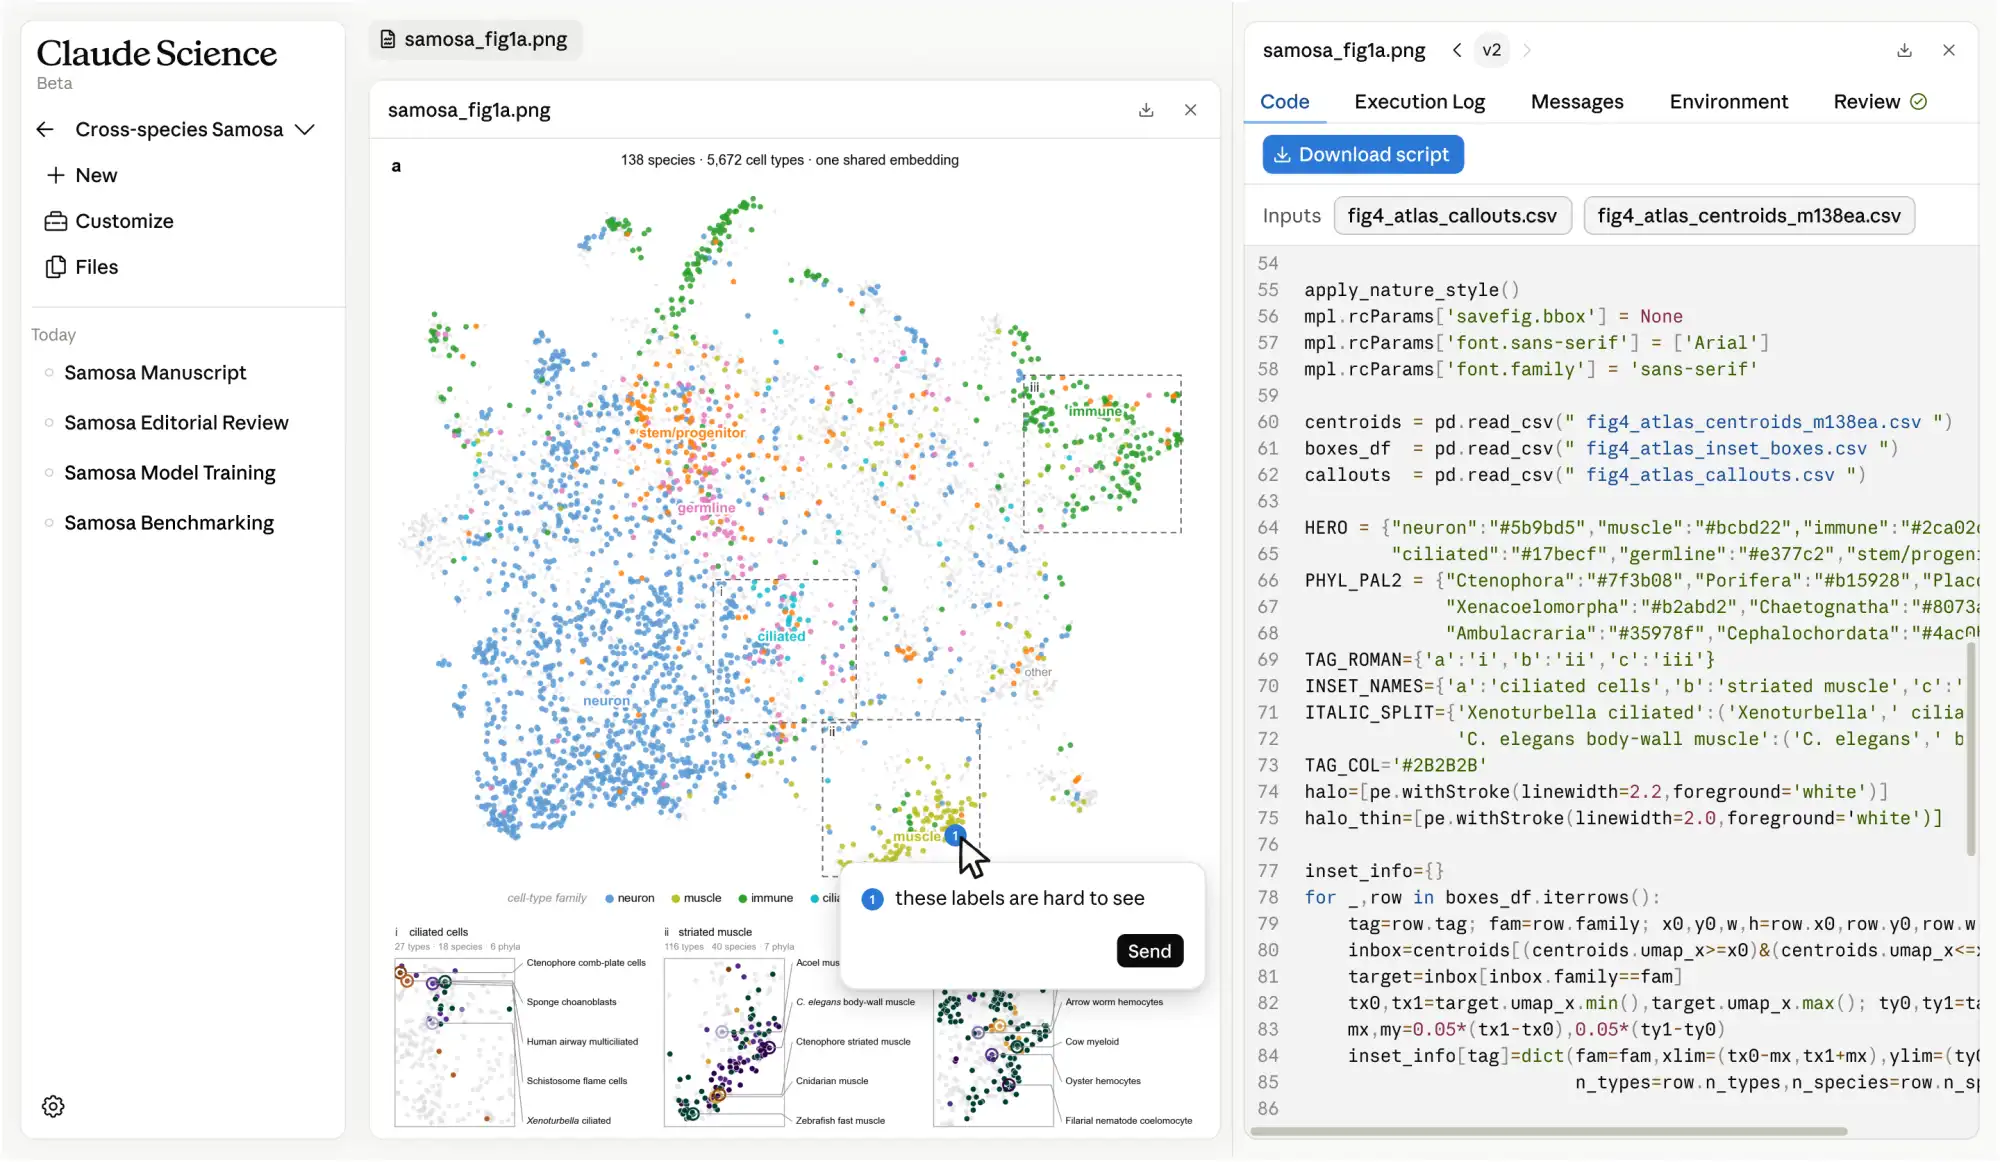
\includegraphics[width=0.8\textwidth]{media/6a43a5d70ebe75212a0ec830_science-pillars-1.png}
\end{center}

\end{document}
